% Options for packages loaded elsewhere
\PassOptionsToPackage{unicode}{hyperref}
\PassOptionsToPackage{hyphens}{url}
%
\documentclass[
]{article}
\usepackage{amsmath,amssymb}
\usepackage{iftex}
\ifPDFTeX
  \usepackage[T1]{fontenc}
  \usepackage[utf8]{inputenc}
  \usepackage{textcomp} % provide euro and other symbols
\else % if luatex or xetex
  \usepackage{unicode-math} % this also loads fontspec
  \defaultfontfeatures{Scale=MatchLowercase}
  \defaultfontfeatures[\rmfamily]{Ligatures=TeX,Scale=1}
\fi
\usepackage{lmodern}
\ifPDFTeX\else
  % xetex/luatex font selection
\fi
% Use upquote if available, for straight quotes in verbatim environments
\IfFileExists{upquote.sty}{\usepackage{upquote}}{}
\IfFileExists{microtype.sty}{% use microtype if available
  \usepackage[]{microtype}
  \UseMicrotypeSet[protrusion]{basicmath} % disable protrusion for tt fonts
}{}
\makeatletter
\@ifundefined{KOMAClassName}{% if non-KOMA class
  \IfFileExists{parskip.sty}{%
    \usepackage{parskip}
  }{% else
    \setlength{\parindent}{0pt}
    \setlength{\parskip}{6pt plus 2pt minus 1pt}}
}{% if KOMA class
  \KOMAoptions{parskip=half}}
\makeatother
\usepackage{xcolor}
\usepackage[margin=1in]{geometry}
\usepackage{longtable,booktabs,array}
\usepackage{calc} % for calculating minipage widths
% Correct order of tables after \paragraph or \subparagraph
\usepackage{etoolbox}
\makeatletter
\patchcmd\longtable{\par}{\if@noskipsec\mbox{}\fi\par}{}{}
\makeatother
% Allow footnotes in longtable head/foot
\IfFileExists{footnotehyper.sty}{\usepackage{footnotehyper}}{\usepackage{footnote}}
\makesavenoteenv{longtable}
\usepackage{graphicx}
\makeatletter
\def\maxwidth{\ifdim\Gin@nat@width>\linewidth\linewidth\else\Gin@nat@width\fi}
\def\maxheight{\ifdim\Gin@nat@height>\textheight\textheight\else\Gin@nat@height\fi}
\makeatother
% Scale images if necessary, so that they will not overflow the page
% margins by default, and it is still possible to overwrite the defaults
% using explicit options in \includegraphics[width, height, ...]{}
\setkeys{Gin}{width=\maxwidth,height=\maxheight,keepaspectratio}
% Set default figure placement to htbp
\makeatletter
\def\fps@figure{htbp}
\makeatother
\setlength{\emergencystretch}{3em} % prevent overfull lines
\providecommand{\tightlist}{%
  \setlength{\itemsep}{0pt}\setlength{\parskip}{0pt}}
\setcounter{secnumdepth}{5}
\ifLuaTeX
  \usepackage{selnolig}  % disable illegal ligatures
\fi
\IfFileExists{bookmark.sty}{\usepackage{bookmark}}{\usepackage{hyperref}}
\IfFileExists{xurl.sty}{\usepackage{xurl}}{} % add URL line breaks if available
\urlstyle{same}
\hypersetup{
  pdftitle={hierarchical\_forecasting\_report},
  pdfauthor={Janice Hsu},
  hidelinks,
  pdfcreator={LaTeX via pandoc}}

\title{hierarchical\_forecasting\_report}
\author{Janice Hsu}
\date{2023-09-30}

\begin{document}
\maketitle

{
\setcounter{tocdepth}{2}
\tableofcontents
}
\begin{itemize}
\tightlist
\item
  Change the accuracy test (the one with 0)
\item
  probably remove the seasonal effect and see if there's a pattern or sth
\end{itemize}

\newpage

\hypertarget{preliminary-analysis}{%
\section{Preliminary Analysis}\label{preliminary-analysis}}

\hypertarget{data-introduction}{%
\subsection{Data Introduction}\label{data-introduction}}

The dataset contains variables related to monthly Emergency Attendances in hospitals in Wales, UK. The data was publicly available and retrieved from StatsWales.

\begin{itemize}
\item
  Data: This column represents the aggregated number of attendances in each emergency department. The data was aggregated according to the other columns.
\item
  YearMonth: This column represents data from 2012 April to 2023 June (135 time points).
\item
  Age\_Code: This column provides the patient's age group. There are 17 different age groups: ``0 to 4'',``5 to 17'',``18 to 24'',``25 to 29'',``30 to 34'',``35 to 39'',``40 to 44'',``45 to 49'',``50 to 54'',``55 to 59'',``60 to 64'',``65 to 69'',``70 to 74'',``75 to 79'',``80 to 84'',``85'' and ``Unknown''.
\item
  Sex\_ItemName\_ENG: This column provides patient's gender using 3 categories: ``Female'', ``Male'' and ``Unknown''.
\item
  Hospital\_Code: This column represents 42 different hospitals in Wales.
\item
  Hospital\_ItemName\_ENG: This columns refers to the name of the 42 different hospitals in Wales.
\item
  Hospital\_Hierarchy: This column represents the code for the health board that the hospital belongs to.
\item
  Hospital\_AltCode1: This column provides an alternate code for the hospital.
\item
  Organisation: This column represents the Local Health Board (LHB), which are responsible for planning and delivering NHS Wales services in their areas, including Emergency Care. In Wales there are 7 distinct LHBs, however two of them, Cwm Taf Morgannwg and Swansea Bay, were previously (before 1 st of April 2019) known as Cwm Taf and Abertawe Bro Morgannwg (therefore this column contains 9 distinct values).
\item
  Organisation\_Code: A code for the organisation as well as the LHB.
\end{itemize}

There are three hierarchies in this dataset:
- On the top level, there is all the hospitals in Wales.
- On the second level, there are the different LHB.
- At the bottom level, there are 42 hospitals.

\newpage

\hypertarget{exploratory-data-analysis}{%
\section{Exploratory Data Analysis}\label{exploratory-data-analysis}}

\hypertarget{number-of-patients-entering-ed-under-different-hospital-hierarchy}{%
\subsection{Number of patients entering ED under different hospital hierarchy}\label{number-of-patients-entering-ed-under-different-hospital-hierarchy}}

\includegraphics{hierarchical_forecasting_files/figure-latex/unnamed-chunk-5-1}

As already mentioned, two LHBs were redefined from the 1st of April 2019 onwards: Cwm Taf ((\# hospitals = 27)--\textgreater{} Cwm Taf Morgannwg ((\# hospitals = 30)// Abertawe Bro Morgannwg ((\# hospitals = 26) --\textgreater{} Swansea Bay ((\# hospitals = 31).

Since the number of hospitals included before and after the change in each LHB was different, these 4 organisations were aggregated into one unique group to enable their inclusion in the forecasting analysis (defined as ``Grouped\_4\_organisation''in the code snippets).

\newpage

\hypertarget{group-the-changed-local-health-board-together}{%
\subsection{Group the changed Local Health Board together}\label{group-the-changed-local-health-board-together}}

\hypertarget{there-are-6-local-health-boards}{%
\subsubsection{There are 6 Local Health Boards}\label{there-are-6-local-health-boards}}

\begin{verbatim}
## [1] "Betsi Cadwaladr"        "Hywel Dda"              "Grouped_4_organisation"
## [4] "Cardiff & Vale"         "Aneurin Bevan"          "Powys Teaching"
\end{verbatim}

\hypertarget{number-of-patients-who-enter-ed-under-6-different-local-health-boards}{%
\subsection{Number of patients who enter ED under 6 different local health boards}\label{number-of-patients-who-enter-ed-under-6-different-local-health-boards}}

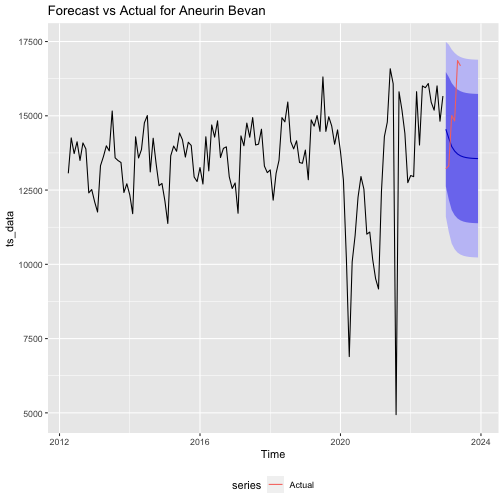
\includegraphics{hierarchical_forecasting_files/figure-latex/unnamed-chunk-9-1}

\textbf{Analysing Health Board Attendance Trends Amidst and Post-COVID-19:}

Healthcare systems around the world faced significant difficulties during the COVID-19 epidemic, which caused them to quickly shift into crisis-response mode. Intriguing trends during and after the epidemic era have been revealed by a thorough review of attendance data from local health boards.

\begin{itemize}
\tightlist
\item
  During the pandemic:
\end{itemize}

Surprisingly, several local health boards experienced a large reduction in attendance throughout the epidemic period. This significant drop in attendance, which may have been brought on by reasons including stringent public health regulations, widespread concern over virus exposure, and maybe changes in healthcare delivery strategies, was an anomalous departure from historical attendance trends.

\begin{itemize}
\tightlist
\item
  Post pandemic:
\end{itemize}

After the pandemic's intensity started to lessen, there was a noticeable increase in attendance, however there were notable differences amongst the local health boards. In contrast to most boards, which showed a strong recovery and raised their attendance figures to levels prior to the pandemic, Powys Teaching stood out as an outlier and defied this recovery trend. To fully understand the subtleties affecting these disparate courses and influence upcoming strategic planning, more research is necessary.

\begin{itemize}
\tightlist
\item
  Findings on seasonality:
\end{itemize}

Initial data analysis reveals the existence of seasonality, which is characterized by repeated swings in attendance across all health boards. This pattern calls for a perceptive investigation into:

Identify Underlying Causes:
Researching seasonality's probable triggers, such as public health initiatives, flu seasons, or holiday seasons, in order to comprehend the factors influencing these patterns.

Determine Seasonal influence:
Establishing whether the observed seasonality has an equal influence on all health boards or whether there are differences, which may be a sign of regional causes or policy changes.

Planning and Forecasting:
By using this understood seasonality to improve forecasting models and ensuring that they are calibrated to account for these seasonal changes, more precise and useful predictive insights are made possible.

\newpage

\hypertarget{seasonality-of-number-of-attendances}{%
\subsection{Seasonality of number of attendances}\label{seasonality-of-number-of-attendances}}

To further explore whether there was any trend and/or seasonality in the data by LHB, the time series was decomposed using the STL method and the extracted components (trend, seasonal and residuals) plotted:

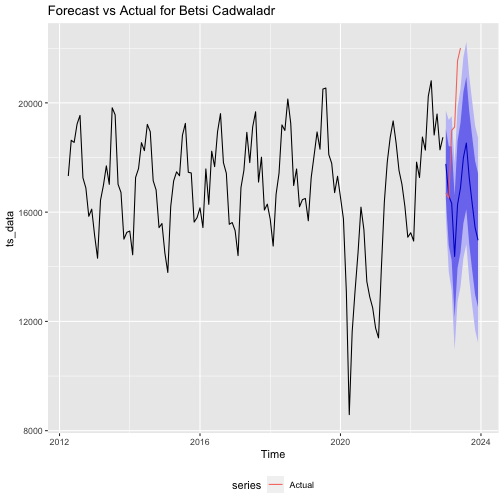
\includegraphics{hierarchical_forecasting_files/figure-latex/unnamed-chunk-10-1}
- Findings:

\begin{enumerate}
\def\labelenumi{\arabic{enumi}.}
\item
  Most LHBs have a trend whereby attendance is lower in some months, like April and November, and higher in others, like June and July.
\item
  In many of the LHBs, the attendance in 2020 differs noticeably from other years.
  In comparison to similar months in past years, the majority of LHBs appear to have a fall or reduction in ED attendances during several months of 2020. This could be a sign of outside influences influencing access to or use of healthcare because of the pandemic.
\item
\end{enumerate}

\begin{itemize}
\tightlist
\item
  Aneurin Bevan: The middle of the year for 2020 shows a clear decline.
\item
  Cardiff \& Vale: Attendances in 2020 appear to be continuously lower than in previous years, particularly in the early months.
\item
  Hywel Dda: Around mid-year, there is a noticeable decline in attendance.
\item
  Betsi Cadwaladr: While the trend for 2020 appears to be largely constant, several months still show a decline in attendance.
\item
  Grouped\_4\_organisation: Attendance clearly drops off during particular months.
\item
  Powys Teaching: The variations are more pronounced, with obvious dips during particular months.
\end{itemize}

\hypertarget{decompose-time-series}{%
\subsubsection{Decompose Time Series}\label{decompose-time-series}}

\hypertarget{plotting}{%
\subsubsection{Plotting}\label{plotting}}

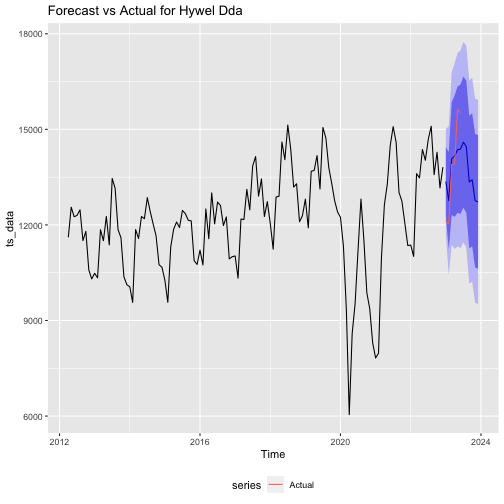
\includegraphics{hierarchical_forecasting_files/figure-latex/unnamed-chunk-14-1}

Findings:

\begin{enumerate}
\def\labelenumi{\arabic{enumi}.}
\item
  Trend:
  There appears to be an upward trend in the number of ED visits over time for all LHBs, but there are outliers.
  The most obvious decline occurs around 2020, which may be a sign of the COVID-19 pandemic's effects.
\item
  Seasonality:
  The seasonal component illustrates the periodicity in ED attendances by showing predictable patterns that repeat annually.
  There is a pronounced surge in the number of patient's attendance in the middle of the year (approximately in June or July). This seasonal pattern underlines the recurrent nature of patient admissions.
\item
  Residuals:
  The residuals are the data's unexplained variation after the trend and seasonal components have been removed.
  The majority of LHBs have residuals that oscillate near zero, which shows that the STL decomposition has effectively caught the main trends in the data.
\end{enumerate}

\newpage

\hypertarget{change-the-age_code-structure-into-different-groups-for-simplicity-and-interpretability}{%
\subsection{Change the Age\_Code structure into different groups for simplicity and interpretability}\label{change-the-age_code-structure-into-different-groups-for-simplicity-and-interpretability}}

\begin{verbatim}
##  [1] "0 to 4"   "18 to 24" "25 to 29" "30 to 34" "35 to 39" "40 to 44"
##  [7] "45 to 49" "5 to 17"  "50 to 54" "55 to 59" "60 to 64" "65 to 69"
## [13] "70 to 74" "75 to 79" "80 to 84" "85"       "Unknown"
\end{verbatim}

\hypertarget{age-group-0-4-5-17-18-69-70}{%
\subsubsection{Age group: ``0-4'', ``5-17'', ``18-69'', ``70\^{}''}\label{age-group-0-4-5-17-18-69-70}}

\hypertarget{plot-number-of-patients-in-different-age-groups}{%
\subsection{Plot Number of Patients in different age groups}\label{plot-number-of-patients-in-different-age-groups}}

\includegraphics{hierarchical_forecasting_files/figure-latex/unnamed-chunk-17-1}

Findings:

\begin{itemize}
\tightlist
\item
  The observation that the age group 18-69 has the most amount of patient attendance is expected, as it is the biggest group among all. However, it is noteworthy that the second biggest group are from the oldest age bracket, aligning with the general understanding of the health care need for the elders.
\end{itemize}

\hypertarget{forecast-with-arima}{%
\section{Forecast with ARIMA}\label{forecast-with-arima}}

\hypertarget{plotting-using-arima}{%
\subsection{Plotting using ARIMA}\label{plotting-using-arima}}

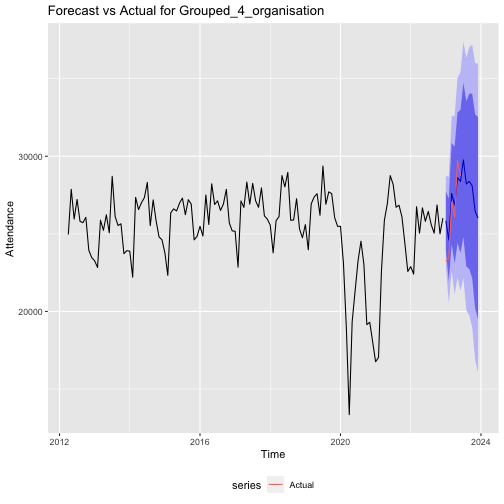
\includegraphics{hierarchical_forecasting_files/figure-latex/unnamed-chunk-23-1}
\includegraphics{hierarchical_forecasting_files/figure-latex/unnamed-chunk-23-2}
\includegraphics{hierarchical_forecasting_files/figure-latex/unnamed-chunk-23-3}
\includegraphics{hierarchical_forecasting_files/figure-latex/unnamed-chunk-23-4}
\includegraphics{hierarchical_forecasting_files/figure-latex/unnamed-chunk-23-5}
\includegraphics{hierarchical_forecasting_files/figure-latex/unnamed-chunk-23-6}
\includegraphics{hierarchical_forecasting_files/figure-latex/unnamed-chunk-23-7}

\hypertarget{forecasting-with-ets}{%
\section{Forecasting with ETS}\label{forecasting-with-ets}}

\hypertarget{plotting-with-ets}{%
\subsection{Plotting with ets}\label{plotting-with-ets}}

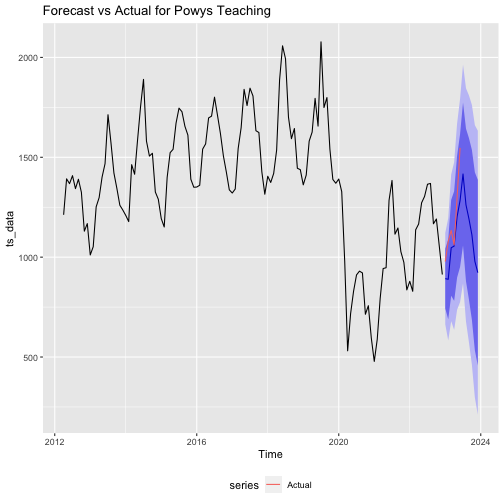
\includegraphics{hierarchical_forecasting_files/figure-latex/unnamed-chunk-25-1}
\includegraphics{hierarchical_forecasting_files/figure-latex/unnamed-chunk-25-2}
\includegraphics{hierarchical_forecasting_files/figure-latex/unnamed-chunk-25-3}
\includegraphics{hierarchical_forecasting_files/figure-latex/unnamed-chunk-25-4}
\includegraphics{hierarchical_forecasting_files/figure-latex/unnamed-chunk-25-5}
\includegraphics{hierarchical_forecasting_files/figure-latex/unnamed-chunk-25-6}
\includegraphics{hierarchical_forecasting_files/figure-latex/unnamed-chunk-25-7}

\begin{itemize}
\tightlist
\item
  Conformity:
\end{itemize}

Hywel Dda, Powys Teaching, Cardiff \& Vale, Grouped\_4\_Organisation, and Total (All-Wales): For these health boards, the ARIMA model effectively predicted the downturn that was observed in the latter portions of 2023 and successfully reflected the actual data, indicating a cogent direction. This demonstrates ARIMA's ability to effectively model and anticipate time-series data for these specific entities, despite the unpredictably fluctuating conditions brought on by the epidemic.

\begin{itemize}
\tightlist
\item
  Contradictions:
\end{itemize}

Aneurin Bevan and Betsi Cadwaladr: By contrast, the prediction statistics for Aneurin Bevan and Betsi Cadwaladr show a clear departure from the actual numbers. It is necessary to assess the ARIMA model's applicability and accuracy with regard to these specific datasets because there is a discrepancy between the predicted value and the real-time data.

\hypertarget{forecasting-with-ets-1}{%
\section{Forecasting with ETS}\label{forecasting-with-ets-1}}

\hypertarget{plotting-with-ets-1}{%
\subsection{Plotting with ets}\label{plotting-with-ets-1}}

\includegraphics{hierarchical_forecasting_files/figure-latex/unnamed-chunk-27-1}
\includegraphics{hierarchical_forecasting_files/figure-latex/unnamed-chunk-27-2}
\includegraphics{hierarchical_forecasting_files/figure-latex/unnamed-chunk-27-3}
\includegraphics{hierarchical_forecasting_files/figure-latex/unnamed-chunk-27-4}
\includegraphics{hierarchical_forecasting_files/figure-latex/unnamed-chunk-27-5}
\includegraphics{hierarchical_forecasting_files/figure-latex/unnamed-chunk-27-6}
\includegraphics{hierarchical_forecasting_files/figure-latex/unnamed-chunk-27-7}

Upon first glance, it appears that the ETS model offers a relatively close alignment with the real data, demonstrating a strong predictive power. When compared to the ARIMA model, the projections closely mimic the actual data patterns rather than merely following them, which suggests a possibility for greater accuracy.

-Consistent Decline in Predictions:

Downtrend in 2023: Regardless of the model used, all forecasts uniformly point to a decline in trends during the second half of 2023. This might be explained by the historical data's apparent cyclical nature. In other words, the historical data reveals a pattern in which peaks frequently appear in the middle of the year and then descend into troughs at year's end and the beginning of the next year. This recurrent pattern may have a significant impact on the expected downturn in 2023.

In light of the above, it is crucial to approach model selection with a nuanced comprehension of the underlying data and impacting factors, even though the ETS model shows a potentially higher prediction accuracy within the given circumstances.

An accuracy analysis was then carried out upon for both ARIMA and ETS models to further assess the quality of their predictions.

\hypertarget{accuracy-assessment-for-arima-and-ets}{%
\section{Accuracy assessment for ARIMA and ETS}\label{accuracy-assessment-for-arima-and-ets}}

\hypertarget{calculating-accuracy-metrics-for-arima-and-ets}{%
\subsection{Calculating Accuracy Metrics for ARIMA and ETS}\label{calculating-accuracy-metrics-for-arima-and-ets}}

\hypertarget{displaying-accuracy-metrics-for-each-column}{%
\subsubsection{Displaying Accuracy Metrics for each Column}\label{displaying-accuracy-metrics-for-each-column}}

\begin{tabular}{l|r|r}
\hline
LHB & ARIMA & ETS\\
\hline
Aneurin Bevan.MAE & 1748.634 & 688.417\\
\hline
Aneurin Bevan.RMSE & 1992.543 & 801.644\\
\hline
Aneurin Bevan.MAPE & 0.113 & 0.048\\
\hline
Betsi Cadwaladr.MAE & 3157.257 & 915.735\\
\hline
Betsi Cadwaladr.RMSE & 3756.403 & 1050.122\\
\hline
Betsi Cadwaladr.MAPE & 0.156 & 0.049\\
\hline
Cardiff \& Vale.MAE & 600.429 & 654.811\\
\hline
Cardiff \& Vale.RMSE & 648.376 & 799.030\\
\hline
Cardiff \& Vale.MAPE & 0.050 & 0.057\\
\hline
Grouped\_4\_organisation.MAE & 1386.277 & 1089.509\\
\hline
Grouped\_4\_organisation.RMSE & 1598.559 & 1315.071\\
\hline
Grouped\_4\_organisation.MAPE & 0.052 & 0.043\\
\hline
Hywel Dda.MAE & 804.597 & 763.085\\
\hline
Hywel Dda.RMSE & 923.853 & 905.503\\
\hline
Hywel Dda.MAPE & 0.058 & 0.059\\
\hline
Powys Teaching.MAE & 238.265 & 120.999\\
\hline
Powys Teaching.RMSE & 264.667 & 146.796\\
\hline
Powys Teaching.MAPE & 0.192 & 0.098\\
\hline
Total.MAE & 4781.817 & 4297.460\\
\hline
Total.RMSE & 5601.875 & 5014.551\\
\hline
Total.MAPE & 0.054 & 0.052\\
\hline
\end{tabular}

\begin{itemize}
\item
  With Cardiff \& Vale being a significant exception, most places displayed reduced error metrics when modeled with ETS, signifying a higher predictive accuracy as compared to the ARIMA model.
\item
  Model Differentiation:
\end{itemize}

ARIMA, A Time-Series Tradition Autoregressive, integrative (difference), and moving average features are included in the forecasting core components.
The foundation is laid by differencing to make data stationary, and then autoregressive and moving average techniques are applied.

ETS: A Comprehensive Method for Time-Series Model Constituent Elements reflects the seasonality, trend, and error components in time series data. Consists of rigorous detection and modeling of error, trend, and seasonal patterns within the data, which tends to include entire pattern analysis.

\begin{itemize}
\tightlist
\item
  According to the interest expressed by the NHS executives, I would like to provide some insights for the error metrics according to the quality of the forecast for the non-zero count data:
\end{itemize}

\begin{enumerate}
\def\labelenumi{\arabic{enumi}.}
\tightlist
\item
  \textbf{Root Mean Squared Error (RMSE)}

  \begin{itemize}
  \tightlist
  \item
    \textbf{Description}: Measures the square root of the average squared differences between forecast and actual values.
  \item
    \textbf{Pros}: It gives more weight to large errors.
  \item
    \textbf{Cons}: It can be influenced significantly by outliers. RMSE might be inflated, if the count data is prone to significant spikes or declines, which should not be the problem for this data except for the Covid-19 era.
  \end{itemize}
\item
  \textbf{Mean Absolute Percentage Error (MAPE)}

  \begin{itemize}
  \tightlist
  \item
    \textbf{Description}: Measures the average of the absolute percentage errors.
  \item
    \textbf{Pros}: It is a relative metric, and is scale-independent and easy to interpret.
  \item
    \textbf{Cons}: MAPE can overemphasize relative errors on small counts.
  \end{itemize}
\item
  \textbf{Mean Absolute Error (MAE)}

  \begin{itemize}
  \tightlist
  \item
    \textbf{Description}: Measures the average of the absolute differences between forecast and actual values.
  \item
    \textbf{Pros}: It's less sensitive to outliers than RMSE. It provides a straightforward average error size.
  \item
    \textbf{Cons}: It does not emphasize large errors.
  \end{itemize}
\end{enumerate}

\textbf{However, RMSE and MAE should not be used for the hierarchical time series data.}
And here is why:

\begin{itemize}
\item
  \textbf{1. Consistency Between Levels:}
  Granularity Errors are not consistently distributed or similar across all hierarchical levels due to the variance in data granularity between levels, and there will be an aggregation dilemma. Due to the variation in magnitude and volume at various hierarchical levels, direct aggregation of RMSE or MAE from bottom levels to top levels might produce inconsistent or biased judgments of forecast accuracy.
\item
  \textbf{2. Problems with reconciliation:}
  It is possible for forecasts to not add up coherently in a hierarchical structure when they are independently generated for several levels. Since they assess mistakes without taking into account hierarchical dependencies, RMSE and MAE do not by default address this reconciliation. And the alignment issue will therefore be caused. The use of standard error measurements at various hierarchical levels may produce false conclusions regarding the precision and dependability of the forecasts in the absence of a cogent reconciliation process.
\item
  \textbf{3. Metric incomparability:}
  Impact of a unit error is not constant across levels; for instance, a 100-unit error may be insignificant at a higher aggregate level but significant at a lower one. Additionally, due to the divergent scales of the errors at various levels, it is difficult to use a single statistic, such as RMSE or MAE, to fairly compare performance across all hierarchical levels.
\end{itemize}

\hypertarget{reconciliation}{%
\section{Reconciliation}\label{reconciliation}}

\hypertarget{aggregate-data}{%
\subsection{Aggregate data}\label{aggregate-data}}

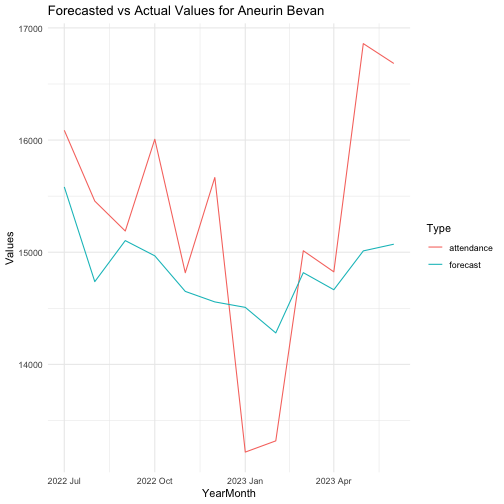
\includegraphics{hierarchical_forecasting_files/figure-latex/unnamed-chunk-37-1}

\hypertarget{time-series-cross-validation}{%
\subsection{Time series cross validation}\label{time-series-cross-validation}}

\hypertarget{stretch_tsibble.init-135-36-.step-1}{%
\subsection{stretch\_tsibble(.init = 135-36, .step = 1)}\label{stretch_tsibble.init-135-36-.step-1}}

135-36-24

data\_gts\_tr \textbar\textgreater{}
model(base = ETS(attendance)) \textbar\textgreater{}
forecast(h = 36)

data\_gts\_fc \textless- data\_gts\_tr \textbar\textgreater{}
model(naive\_model = NAIVE(attendance),
ets\_model = ETS(attendance),
tscount = TSCOUNT(attendance \textasciitilde{} trend() + season() , link = ``log'', model = list(past\_obs = 1:12))) \textbar\textgreater{}
forecast(h = 36)

\hypertarget{tscv-accuracy}{%
\section{TSCV accuracy}\label{tscv-accuracy}}

tscv\_model \textless- data\_gts\_tr \textbar\textgreater{}
model(
naive\_model = NAIVE(attendance),
ets\_model = ETS(attendance),
tscount = TSCOUNT(attendance \textasciitilde{} trend() + season() , link = ``log'', model = list(past\_obs = 1:12))
)\textbar\textgreater{} mutate (comb = (naive\_model+ets\_model+tscount)/3)

\hypertarget{function-to-calculate-mase-and-rmsse-for-a-single-model}{%
\section{Function to calculate MASE and RMSSE for a single model}\label{function-to-calculate-mase-and-rmsse-for-a-single-model}}

calc\_scaled\_errors\_for\_model\_organisation \textless- function(model\_name, organisation) \{
\# Get forecasted and actual values for specific model and organisation
fc\_single\_model\_org \textless- tscv\_model \%\textgreater\%
forecast(h = 36) \%\textgreater\%
filter(.model == model\_name, Aggregated\_Organisation == organisation)

forecasted\_values\_single \textless- fc\_single\_model\_org\$.mean

actual\_values\_org \textless- test\_data \%\textgreater\%
filter(Aggregated\_Organisation == organisation) \%\textgreater\%
pull(attendance)

\# Calculate errors
errors \textless- actual\_values\_org - forecasted\_values\_single
mean\_abs\_error \textless- mean(abs(errors), na.rm = TRUE)
mean\_squared\_error \textless- mean(errors\^{}2, na.rm = TRUE)

\# Calculate naive errors using direct indexing for lag
naive\_forecast \textless- c(NA, actual\_values\_org{[}1:(length(actual\_values\_org) - 1){]}) \# Shift the series by one
naive\_errors \textless- actual\_values\_org - naive\_forecast
naive\_forecast\_error \textless- mean(abs(naive\_errors), na.rm = TRUE) \# For MASE
naive\_forecast\_squared\_error \textless- mean(naive\_errors\^{}2, na.rm = TRUE) \# For RMSSE

\# Calculate MASE and RMSSE
MASE \textless- mean\_abs\_error / naive\_forecast\_error
RMSSE \textless- sqrt(mean\_squared\_error / naive\_forecast\_squared\_error) \# This is a hypothesized version of RMSSE based on MASE's concept

return(list(MASE = MASE, RMSSE = RMSSE))
\}

\hypertarget{specify-models-and-organisations}{%
\section{Specify models and organisations}\label{specify-models-and-organisations}}

models \textless- c(``naive\_model'', ``ets\_model'', ``tscount'', ``comb'')
organisations \textless- unique(training\_data\$Aggregated\_Organisation)

\hypertarget{nested-lapply-to-iterate-over-models-and-organisations}{%
\section{Nested lapply to iterate over models and organisations}\label{nested-lapply-to-iterate-over-models-and-organisations}}

results\_list \textless- lapply(models, function(model) \{
model\_results \textless- lapply(organisations, function(org) \{
calc\_scaled\_errors\_for\_model\_organisation(model, org)
\})

\# Name each element in the list for clarity
names(model\_results) \textless- organisations

\# Include the model name in the results
return(list(
model = model,
results = model\_results
))
\})

\hypertarget{set-names-for-the-list-based-on-model-names-for-clarity}{%
\section{Set names for the list based on model names for clarity}\label{set-names-for-the-list-based-on-model-names-for-clarity}}

names(results\_list) \textless- models

\hypertarget{define-safe_extract-function}{%
\section{Define safe\_extract function}\label{define-safe_extract-function}}

safe\_extract \textless- function(x, field) \{
if (is.list(x) \&\& !is.null(x{[}{[}field{]}{]})) \{
return(x{[}{[}field{]}{]})
\} else \{
return(NA)
\}
\}

\hypertarget{convert-the-results-list-to-a-data-frame}{%
\section{Convert the results list to a data frame}\label{convert-the-results-list-to-a-data-frame}}

results\_df \textless- map\_df(results\_list, \textasciitilde\{
if (is.list(.x\(results)) {  map_df(.x\)results, \textasciitilde\{
tibble(
organisation = names(.x),
MASE = safe\_extract(.x, ``MASE''),
RMSSE = safe\_extract(.x, ``RMSSE'')
)
\}, .id = ``model'')
\} else \{
return(tibble(organisation = NA, MASE = NA, RMSSE = NA, model = NA))
\}
\}, .id = ``model\_name'')

\hypertarget{selecting-relevant-columns}{%
\section{Selecting relevant columns}\label{selecting-relevant-columns}}

results\_df \textless- results\_df \%\textgreater\%
select(model\_name, model, organisation, MASE, RMSSE) \%\textgreater\%
filter(model == ``'')

\hypertarget{print-the-results}{%
\section{Print the results}\label{print-the-results}}

print(results\_df)

\begin{itemize}
\item
  Base Forecasting: This technique is used to forecast straightforward time series data. Using statistical or machine learning models to extrapolate future data points based on observed past data is the main focus of this technique. Base forecasting, which is frequently applied when dealing with a single time series, tries to find patterns, trends, and seasonality in the historical data in order to produce precise and trustworthy future projections.
\item
  Reconciliation Forecasting (Hierarchical Forecasting): Reconciliation or Hierarchical forecasting is typically used when managing hierarchical or grouped time series data. It involves generating forecasts on several levels of aggregation. This process not only creates projections for each individual time series, but also reconciles the forecasts to guarantee consistency throughout the hierarchy's many levels. The forecasts may be distributed across hierarchical levels using a variety of strategies, such as top-down, bottom-up, to make sure that the projections at each level coincide with their corresponding aggregate levels. When the data contains a hierarchical structure, such as organisational, product, or geographic hierarchies, hierarchical forecasting is especially advantageous since it ensures consistent and consolidated projections at all levels.
\end{itemize}

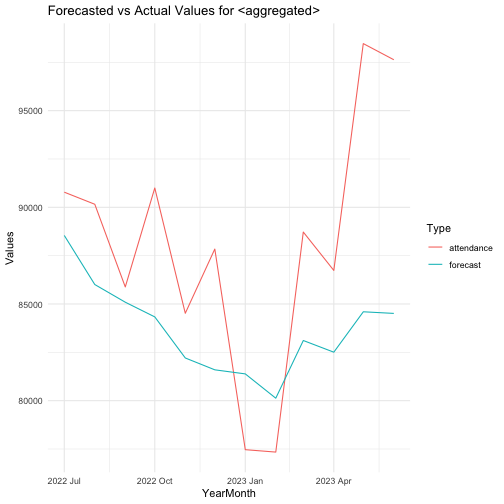
\includegraphics{hierarchical_forecasting_files/figure-latex/unnamed-chunk-41-1}

\end{document}
